\documentclass{article}

\usepackage{enumitem}
\usepackage{fontspec}
\usepackage[letterpaper,margin=72pt]{geometry}
\usepackage{hyperref}
\usepackage{import}
\usepackage{listings}
\usepackage{xcolor}

\subimport{../}{colors.tex}

\setsansfont{Overpass}[Scale=MatchLowercase]
\setmonofont{Overpass Mono}[Scale=MatchLowercase]

\renewcommand{\familydefault}{\sfdefault}

\hypersetup{
  colorlinks=true,
  urlcolor=uclablue,
}

\setlist{nosep}

\makeatletter
\newcommand\version[1]{\renewcommand\@version{#1}}
\newcommand\@version{}

\newcommand\labnumber[1]{\renewcommand\@labnumber{#1}}
\newcommand\@labnumber{}

\newcommand\duedate[1]{\renewcommand\@duedate{#1}}
\newcommand\@duedate{}

\renewcommand\maketitle{%
  \noindent
  {\Large \color{uclablue} CS 111: Operating System Principles}

  \noindent
  {\Large \color{uclablue} Lab \@labnumber}\\[-0.75em]

  \noindent
  {\Huge \bfseries \color{uclablue} \@title}
  {\ttfamily \footnotesize \color{uclablue} \@version}\\[-0.75em]

  \noindent
  {\@author}

  \noindent
  {\@date}

  \noindent
  {Due: \@duedate}\\[1em]
}
\makeatother

\lstset{
  basicstyle=\ttfamily,
}


\lecturenumber{2}
\title{Interfaces}
\version{2.0.0}
\author{Jon Eyolfson}
\date{June 24, 2021}

\begin{document}

  \begin{frame}[plain, noframenumbering]
    \titlepage
  \end{frame}

  \begin{frame}
    \frametitle{CPUs Have ``Rings'' to Control Instruction Access}

    \centering
    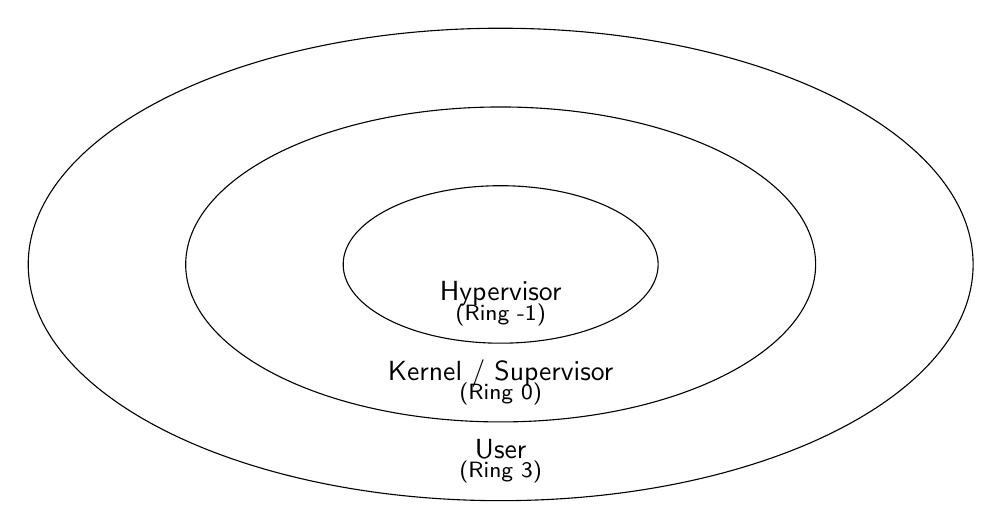
\begin{tikzpicture}
      \draw (0,0) ellipse (2cm and 1cm);
      \draw (0,0) ellipse (4cm and 2cm);
      \draw (0,0) ellipse (6cm and 3cm);
      \node [align=center] at (0, -0.5) {
        Hypervisor \\[-0.5em] \footnotesize (Ring -1)
      };
      \node [align=center] at (0, -1.5) {
        Kernel / Supervisor \\[-0.5em] \footnotesize (Ring 0)
      };
      \node [align=center] at (0, -2.5) {
        User \\[-0.5em] \footnotesize (Ring 3)
      };
    \end{tikzpicture}

    \begin{flushright}
      Each ring can access instructions in any of its outer rings
    \end{flushright}
  \end{frame}

  \begin{frame}
    \frametitle{The Kernel of the Operating System Runs in Kernel Mode}

    \begin{tikzpicture}
      \draw [primarycolor, dashed, thick] (0,0) -- ($(\textwidth - 3pt, 0)$);
      \node [primarycolor, anchor=south east] at ($(\textwidth - 3pt, 0)$)
            (user) {User space};
      \node [primarycolor, anchor=north east] at ($(\textwidth - 3pt, 0)$)
            (kernel) {Kernel space};
    \end{tikzpicture}
  \end{frame}

  \begin{frame}
    \frametitle{System Calls Transition between User and Kernel Mode}

    \begin{tikzpicture}
      \draw [primarycolor, dashed, thick] (0,0.75) -- ($(\textwidth - 3pt, 0.75)$);
      \node [primarycolor, anchor=south east] at ($(\textwidth - 3pt, 0.75)$)
            (user) {User space};
      \draw [primarycolor, dashed, thick] (0,-0.75) -- ($(\textwidth - 3pt, -0.75)$);
      \node [primarycolor, anchor=north east] at ($(\textwidth - 3pt, -0.75)$)
            (kernel) {Kernel space};
      \node [anchor=east] at ($(\textwidth - 3pt, -0)$) {\footnotesize (352 total)};
      \node [align=center] at ($(\textwidth/2 - 1.5pt, 0)$)
        {\footnotesize\ttfamily read write open close stat mmap brk pipe clone fork \\
         \footnotesize\ttfamily execve exit wait4 chdir  mkdir rmdir creat mount \\
         \footnotesize\ttfamily init\_module delete\_module clock\_nanosleep exit\_group };
    \end{tikzpicture}
  \end{frame}

  \begin{frame}
    \frametitle{A Monolithic Kernel Runs Operating System Services in Kernel Mode}

    \begin{tikzpicture}[box/.style={draw, minimum width=3.5cm, minimum height=2em,
                                    inner sep=0.5em, node distance=0.5cm}]
      \draw [primarycolor, dashed, thick] (0,0) -- ($(\textwidth - 3pt, 0)$);
      \node [primarycolor, anchor=south east] at ($(\textwidth - 3pt, 0)$)
            (user) {User space};
      \node [primarycolor, anchor=north east] at ($(\textwidth - 3pt, 0)$)
            (kernel) {Kernel space};
      \node [box] (sched) at ($(\textwidth/2 - 1.5pt, -1.25)$) {Process Scheduling};
      \node [box, left=of sched] {Virtual Memory};
      \node [box, right=of sched] {IPC};
      \node [box, below=of sched] (dd) {Device Drivers};
      \node [box, left=of dd] {File Systems};
    \end{tikzpicture}
  \end{frame}

  \begin{frame}
    \frametitle{A Microkernel Runs the Minimum Amount of Services in Kernel Mode}

    \begin{tikzpicture}[box/.style={draw, minimum width=3.5cm, minimum height=2em,
                                    inner sep=0.5em, node distance=0.5cm}]
      \draw [primarycolor, dashed, thick] (0,0) -- ($(\textwidth - 3pt, 0)$);
      \node [primarycolor, anchor=south east] at ($(\textwidth - 3pt, 0)$)
            (user) {User space};
      \node [primarycolor, anchor=north east] at ($(\textwidth - 3pt, 0)$)
            (kernel) {Kernel space};
      \node [box] (sched) at ($(\textwidth/2 - 1.5pt, -1.25)$) {Process Scheduling};
      \node [box, left=of sched] {Virtual Memory};
      \node [box, right=of sched] {Basic IPC};
      \node [box] (dd) at ($(\textwidth/2 - 1.5pt, 1.25)$) {Device Drivers};
      \node [box, left=of dd] {File Systems};
      \node [box, right=of dd] {Advanced IPC};
    \end{tikzpicture}
  \end{frame}

  \begin{frame}
    \frametitle{Other Types of Kernels}

    ``Hybrid'' kernels are between monolithic and microkernels

    \hspace{2em} Emulation services to user mode (Windows)

    \hspace{2em} Device drivers to user mode (macOS)

    \vspace{2em}

    Nanokernels and picokernels

    \hspace{2em} Move even more into user mode than traditional microkernels

    \vspace{4em}

    There's many different lines you can draw with different trade-offs
  \end{frame}

  \begin{frame}
    \frametitle{Let's Execute a 178 Byte ``Hello World'' on Linux x86-64}

    \scriptsize \ttfamily
    0x7F 0x45 0x4C 0x46 0x02 0x01 0x01 0x03 0x00 0x00 0x00 0x00 0x00 0x00 0x00
    0x00

    0x02 0x00 0x3E 0x00 0x01 0x00 0x00 0x00 0x78 0x00 0x01 0x00 0x00 0x00 0x00
    0x00

    0x40 0x00 0x00 0x00 0x00 0x00 0x00 0x00 0x00 0x00 0x00 0x00 0x00 0x00 0x00
    0x00

    0x00 0x00 0x00 0x00 0x40 0x00 0x38 0x00 0x01 0x00 0x40 0x00 0x00 0x00 0x00
    0x00

    0x01 0x00 0x00 0x00 0x05 0x00 0x00 0x00 0x00 0x00 0x00 0x00 0x00 0x00 0x00
    0x00

    0x00 0x00 0x01 0x00 0x00 0x00 0x00 0x00 0x00 0x00 0x01 0x00 0x00 0x00 0x00
    0x00

    0xB2 0x00 0x00 0x00 0x00 0x00 0x00 0x00 0xB2 0x00 0x00 0x00 0x00 0x00 0x00
    0x00

    0x00 0x01 0x00 0x00 0x00 0x00 0x00 0x00 0x48 0xC7 0xC0 0x01 0x00 0x00 0x00
    0x48

    0xC7 0xC7 0x01 0x00 0x00 0x00 0x48 0xC7 0xC6 0xA6 0x00 0x01 0x00 0x48 0xC7
    0xC2

    0x0C 0x00 0x00 0x00 0x0F 0x05 0x48 0xC7 0xC0 0xE7 0x00 0x00 0x00 0x48 0xC7
    0xC7

    0x00 0x00 0x00 0x00 0x0F 0x05 0x48 0x65 0x6C 0x6C 0x6F 0x20 0x77 0x6F 0x72
    0x6C

    0x64 0x0A
  \end{frame}

  \begin{frame}
    \frametitle{ELF is the Binary Format for Unix Operating Systems}

    Executable and Linkable Format (ELF) is a file format

    \vspace{2em}

    Always starts with the 4 bytes: \hspace{0.5em} \texttt{0x7F 0x45 0x4C 0x46}

    \hspace{3em} or with ASCII encoding: \hspace{0.5em}
    \texttt{0x7F~~'E'~~'L'~~'F'}

    \vspace{2em}

    Followed by a byte signifying 32 or 64 bit architectures

    \hspace{2em} then a byte signifying little or big endian

    \vspace{4em}

    Most file formats have different starting signatures (or magic numbers)
  \end{frame}

  \begin{frame}
    \frametitle{Use \texttt{readelf} to Read ELF File Headers}

    Command: \hspace{0.5em} \texttt{readelf <filename>}

    \vspace{1em}

    Contains the following:
    \begin{itemize}
      \item Information about the machine (e.g. the ISA)
      \item The entry point of the program
      \item Any \structure{program headers} (required for executables)
      \item Any \structure{section headers} (required for libraries)
    \end{itemize}

    \vspace{2em}

    The header is 64 bytes, so we still have to account for 114 more.
  \end{frame}

  \begin{frame}[fragile]
    \frametitle{Result of \texttt{readelf -h} on ``Hello world''}

    \begin{lstlisting}[basicstyle=\scriptsize\ttfamily]
ELF Header:
  Magic:   7f 45 4c 46 02 01 01 03 00 00 00 00 00 00 00 00 
  Class:                             ELF64
  Data:                              2's complement, little endian
  Version:                           1 (current)
  OS/ABI:                            UNIX - GNU
  ABI Version:                       0
  Type:                              EXEC (Executable file)
  Machine:                           Advanced Micro Devices X86-64
  Version:                           0x1
  Entry point address:               0x10078
  Start of program headers:          64 (bytes into file)
  Start of section headers:          0 (bytes into file)
  Flags:                             0x0
  Size of this header:               64 (bytes)
  Size of program headers:           56 (bytes)
  Number of program headers:         1
  Size of section headers:           64 (bytes)
  Number of section headers:         0
  Section header string table index: 0
    \end{lstlisting}
  \end{frame}

  \begin{frame}
    \frametitle{ELF Program Header}

    Tells the operating system how to load the executable:

    \begin{itemize}
      \item Which type? Examples:
        \begin{itemize}
          \item Load directly into memory
          \item Use dynamic linking (libraries)
          \item Interpret the program
        \end{itemize}
      \item Permissions? Read / Write / Execute
      \item Which virtual address to put it?
        \begin{itemize}
          \item Note that you'll rarely ever use physical addresses (for embedded)
        \end{itemize}
    \end{itemize}

    \vspace{2em}

    For ``Hello world'' we load everything into memory

    \hspace{2em} One program header is 56 bytes

    \hspace{4em} 58 bytes left
  \end{frame}

  \begin{frame}[fragile]
    \frametitle{Result of \texttt{readelf -l} on ``Hello world''}

    \begin{lstlisting}[basicstyle=\scriptsize\ttfamily]
Elf file type is EXEC (Executable file)
Entry point 0x10078
There is 1 program header, starting at offset 64

Program Headers:
  Type           Offset             VirtAddr           PhysAddr
                 FileSiz            MemSiz              Flags  Align
  LOAD           0x0000000000000000 0x0000000000010000 0x0000000000010000
                 0x00000000000000b2 0x00000000000000b2  R E    0x100
    \end{lstlisting}
  \end{frame}

  \begin{frame}[fragile]
    \frametitle{``Hello world'' Needs 2 System Calls}

    Command: \hspace{0.5em} \texttt{strace <filename>}

    \vspace{2em}
    
    This shows all the system calls our program makes:

    \vspace{2em}

    \begin{lstlisting}[basicstyle=\scriptsize\ttfamily]
execve("./hello_world", ["./hello_world"], 0x7ffd0489de40 /* 46 vars */) = 0
write(1, "Hello world\n", 12)           = 12
exit_group(0)                           = ?
+++ exited with 0 +++
    \end{lstlisting}
  \end{frame}

  \begin{frame}
    \frametitle{Quick Aside: API Tells You What and ABI Tells You How} 

    Application Programming Interface (API) abstracts the details how how to
    communicate

    \vspace{2em}

    \hspace{2em} e.g. A function takes 2 integer arguments

    \vspace{4em}

    Application Binary Interface (ABI) specifies how to layout data and how to
    concretely communicate

    \vspace{2em}

    \hspace{2em} e.g. The same function using the C calling convention
  \end{frame}

  \begin{frame}
    \frametitle{System Call API for ``Hello world''}

    \texttt{strace} shows the API of system calls

    \vspace{2em}

    The \texttt{write} system call's API is:
    \begin{itemize}
      \item A file descriptor to write bytes to
      \item An address to contiguous sequence of bytes
      \item How many bytes to write from the sequence
    \end{itemize}
    
    \vspace{2em}

    The \texttt{exit\_group} system call's API is:
    \begin{itemize}
      \item An exit code for the program (0-255)
    \end{itemize}
  \end{frame}

  \begin{frame}
    \frametitle{System Call ABI for Linux x86-64}

    Enter the kernel with a \texttt{syscall} instruction, using registers for
    arguments:

    \begin{itemize}
      \item \texttt{rax} --- System call number
      \item \texttt{rdi} --- 1\textsuperscript{st} argument
      \item \texttt{rsi} --- 2\textsuperscript{nd} argument
      \item \texttt{rdx} --- 3\textsuperscript{rd} argument
      \item \texttt{r10} --- 4\textsuperscript{th} argument
      \item \texttt{r8} --- 5\textsuperscript{th} argument
      \item \texttt{r9} --- 6\textsuperscript{th} argument
    \end{itemize}

    What are the limitations of this?

    \vspace{2em}

    Note: other registers are not used, whether they're saved isn't important
    for us
  \end{frame}

  \begin{frame}[fragile]
    \frametitle{Instructions for ``Hello world'', Using the Linux x86-64 ABI}

    Plug in the next 46 bytes into a disassembler, such as:
    \url{https://onlinedisassembler.com/}

    \vspace{2em}

    Our disassembled instructions:
    \begin{lstlisting}[xleftmargin=2em]
mov rax,0x1
mov rdi,0x1
mov rsi,0x100a6
mov rdx,0xc
syscall
mov rax,0xe7
mov rdi,0x0
syscall
    \end{lstlisting}
  \end{frame}

  \begin{frame}
    \frametitle{Finishing Up ``Hello world'' Example}

    The remaining 12 bytes is the ``Hello world'' string itself, ASCII encoded:
    
    \texttt{\footnotesize 0x48 0x65 0x6C 0x6C 0x6F 0x20 0x77 0x6F 0x72 0x6C 0x64 0x0A}

    \vspace{2em}

    \hspace{2em} Low level ASCII tip: bit 5 is \texttt{0}/\texttt{1} for upper
    case/lower case (values differ by 32)

    \vspace{2em}

    This accounts for every single byte of our 178 byte program, let's see what
    C does...

    \vspace{2em}
    Can you already spot a difference between strings in our example compared to
    C?
  \end{frame}

  \begin{frame}[fragile]
    \frametitle{Source Code for ``Hello world'' in C}

    \begin{lstlisting}
#include <stdio.h>

int main(int argc, char **argv)
{
  printf("Hello world\n");
  return 0;
}
    \end{lstlisting}

    Compile with \lstinline|Make| in \lstinline|examples/lecture-02|

    \vspace{2em}

    What are other notable differences between this and our ``Hello world''?
  \end{frame}

  \begin{frame}[fragile]
    \frametitle{System Calls for ``Hello world'' in C, Finding Standard Library}
    \begin{lstlisting}[basicstyle=\ttfamily\scriptsize]
execve("./hello_world_c", ["./hello_world_c"], 0x7ffcb3444f60 /* 46 vars */) = 0
brk(NULL)                               = 0x5636ab9ea000
openat(AT_FDCWD, "/etc/ld.so.cache", O_RDONLY|O_CLOEXEC) = 3
fstat(3, {st_mode=S_IFREG|0644, st_size=149337, ...}) = 0
mmap(NULL, 149337, PROT_READ, MAP_PRIVATE, 3, 0) = 0x7f4d43846000
close(3)                                = 0
openat(AT_FDCWD, "/usr/lib/libc.so.6", O_RDONLY|O_CLOEXEC) = 3
read(3, "\177ELF\2\1\1\3\0\0\0\0\0\0\0\0\3\0>\0\1\0\0\0000C"..., 832) = 832
lseek(3, 792, SEEK_SET)                 = 792
read(3, "\4\0\0\0\24\0\0\0\3\0\0\0GNU\0\201\336\t\36\251c\324"..., 68) = 68
fstat(3, {st_mode=S_IFREG|0755, st_size=2136840, ...}) = 0
mmap(NULL, 8192, PROT_READ|PROT_WRITE, MAP_PRIVATE|MAP_ANONYMOUS, -1, 0)
  = 0x7f4d43844000
lseek(3, 792, SEEK_SET)                 = 792
read(3, "\4\0\0\0\24\0\0\0\3\0\0\0GNU\0\201\336\t\36\251c\324"..., 68) = 68
lseek(3, 864, SEEK_SET)                 = 864
read(3, "\4\0\0\0\20\0\0\0\5\0\0\0GNU\0\2\0\0\300\4\0\0\0\3\0\0", 32) = 32
    \end{lstlisting}
  \end{frame}

  \begin{frame}[fragile]
    \frametitle{System Calls for ``Hello world'' in C, Loading Standard Library}

    \begin{lstlisting}[basicstyle=\ttfamily\scriptsize]
mmap(NULL, 1848896, PROT_READ, MAP_PRIVATE|MAP_DENYWRITE, 3, 0) = 0x7f4d43680000
mprotect(0x7f4d436a2000, 1671168, PROT_NONE) = 0
mmap(0x7f4d436a2000, 1355776, PROT_READ|PROT_EXEC,
  MAP_PRIVATE|MAP_FIXED|MAP_DENYWRITE, 3, 0x22000) = 0x7f4d436a2000
mmap(0x7f4d437ed000, 311296, PROT_READ,
  MAP_PRIVATE|MAP_FIXED|MAP_DENYWRITE, 3, 0x16d000) = 0x7f4d437ed000
mmap(0x7f4d4383a000, 24576, PROT_READ|PROT_WRITE,
  MAP_PRIVATE|MAP_FIXED|MAP_DENYWRITE, 3, 0x1b9000) = 0x7f4d4383a000
mmap(0x7f4d43840000, 13888, PROT_READ|PROT_WRITE,
  MAP_PRIVATE|MAP_FIXED|MAP_ANONYMOUS, -1, 0) = 0x7f4d43840000
close(3)                                = 0
arch_prctl(ARCH_SET_FS, 0x7f4d43845500) = 0
mprotect(0x7f4d4383a000, 16384, PROT_READ) = 0
mprotect(0x5636a9abd000, 4096, PROT_READ) = 0
mprotect(0x7f4d43894000, 4096, PROT_READ) = 0
munmap(0x7f4d43846000, 149337)          = 0
fstat(1, {st_mode=S_IFCHR|0620, st_rdev=makedev(0x88, 0x1), ...}) = 0
    \end{lstlisting}
  \end{frame}

  \begin{frame}[fragile]
    \frametitle{System Calls for ``Hello world'' in C, Setting Up Heap and
                Printing}

    \begin{lstlisting}
brk(NULL)                               = 0x5636ab9ea000
brk(0x5636aba0b000)                     = 0x5636aba0b000
write(1, "Hello world\n", 12)           = 12
exit_group(0)                           = ?
+++ exited with 0 +++
    \end{lstlisting}

    \vspace{1em}
    The C version of ``Hello world'' ends with the exact same system calls we
    made
  \end{frame}

  \begin{frame}
    \frametitle{You Can Think of the Kernel as a Long Running Process}

    Writing kernel code is more like writing library code (there's no \texttt{main})

    \vspace{2em}

    The kernel lets you load code (called modules)

    \vspace{2em}

    Your code executes on-demand

    \hspace{2em} e.g. when it's loaded, or accessing a certain file

    \vspace{2em}

    Remember, your kernel module can execute privileged instructions

    \hspace{2em} and access any kernel data, so you could do anything
  \end{frame}

  \begin{frame}
    \frametitle{Kernel Interfaces Operate Between CPU Mode Boundaries}

    The lessons from the lecture:
    \begin{itemize}
      \item Code running in kernel mode is part of your kernel
      \item Different kernel architectures shift how much code runs in kernel mode
      \item System calls are the interface between user and kernel mode
        \begin{itemize}
          \item Every program must use this interface!
        \end{itemize}
      \item File format and instructions to define a simple ``Hello world'' (in 178 bytes)
        \begin{itemize}
          \item Difference between API and ABI
          \item How to explore system calls
        \end{itemize}
    \end{itemize}
  \end{frame}

\end{document}
